% !TeX root = ../AdaptiveSeedingSTOC.tex

In this section we evaluate the ability of the optimizer to optimize 
a single parameter in the DFC algorithm with respect to very simple 
utility functions and budgets. We test the optimizer on both synthetic 
and real-world datsets and conclude that most of the time it performs 
as well as the best manual parameter settings. 

\subsection{Methodology}

We evaluate the optimizer on both Gaussian Random matrices and the 
Movielens10M dataset 
(available at \url{http://grouplens.org/datasets/movielens/}). 
For each of the two datasets, we divided the available data 
into several partitions. For the random matrices we used five 
partitions, and this simply meant one matrix per partition. 
For the Movielens data (which is one enormous matrix), we 
partitioned the rows of the matrix into seven pieces (meaning, we 
subdivided the data into groups of users). 
This gave the two datasets a comparable number of nonzero entries 
per partition. 

After partitioning the data, we group the partitions into training 
data and testing data. We used all but one partition for both datasets 
as training data on which to run DFC computations. The optimizer was 
then fed the input and output profiles of these computations to use 
in its database. We used the final partition to test the predictions 
of the optimizer. 

Our goal was for the optimizer to automatically choose the degree 
of parallelism in the DFC algorithm, i.e. how much to slice the 
input matrix in the Divide step. We asked for the computations to 
be completed within a specified amount of time while minimizing the 
error, and DFC computations with manually-chosen parameters designed 
to meet these budgets were performed on this testing data, as well as 
a DFC computation with optimizer-chosen division. Error was computed 
using the Root Mean Square Error (RMSE) of the returned factorization 
compared to the revealed entries, and the time of a computation is 
defined as the maximum time of a slice computation plus the time 
it takes to finish the projection step of DFC.  

The evaluation metric we chose was, for each time budget, the error 
of the optimized parameters compared to the error of the \emph{best} 
run with manually-chosen parameters. We define the \emph{regret} 
of the optimizer on these instances as the average over the budgets 
of the percent difference in error of the optimized and manual parameters. 
We will see soon that the optimizer performs as well as the best parameter 
for every budget, even when that parameter changes depending on the 
budget. Finally, we performed cross-validation, i.e. training and 
testing was done with each of the partitions used as testing data, 
and we obtain very consistent results. 

We implemented the DFC algorithm in SparkR \cite{V13}, and the optimizer 
in Python. All of our tests were performed on the Amazon EC2 Cluster 
using medium instances. 

\subsection{Gaussian Random Matrices}
The first dataset we tested the optimizer on was a synthetic 
dataset containing many low rank randomly generated matrices. 
The matrices were generated according to the following procedure: 
\begin{enumerate}
\item Fix parameters $r$, $p$, and $\sigma^2$ which are the rank, 
percent of revealed entries, and the variance of the noise respectively.
\item Generate two $n \times r$ matrices ${\bf A}$ and ${\bf B}$ with 
entries drawn from $\mathcal{N}(0,1/\sqrt{r})$. 
\item Let ${\bf N}$ be an $n \times n$ matrix with ${\bf N}(i,j)$ drawn 
independently from $\mathcal{N}(0,\sigma^2)$. 
\item Define ${\bf M} = {\bf A}{\bf B}^T + {\bf N}$
\item Pick a uniform random subset $\Omega \subset [n] \times [n]$ 
with $|\Omega| = pn^2$, and let ${\bf M}_{\Omega}$ be the matrix such 
that ${\bf M}_{\Omega}(i,j) = {\bf M}$ for $(i,j) \in \Omega$ and 
unknown otherwise. 
\end{enumerate}
This procedure generates a noisy copy of a rank $r$ random matrix 
whose entries have unit variance and hides most of its entries. 
Now we can generate many of these matrices and by running a lot of 
DFC computations for training purposes, we can predict the behavior 
of DFC on these kinds of instances and thus automatically 
choose how much to divide the input. 

We generated five $4000 \times 4000$ matrices with 
\[(r,p,\sigma^2) = (10,.1,.01),\] 
and split the data into training/testing splits as mentioned 
in the previous section. Figure \ref{fig:4ktraintest} displays the 
results of one of the training/testing splits of the data. 
Each curve of the graph represents a choice of the division parameter 
in DFC. The first graph is the training data and we can empirically 
see that there are specific intersection points where the parameter 
choice should change. The second graph shows the error of DFC 
computations with manually chosen and optimized parameters. 
Each curve represents a specific choice of the division parameter, 
and the bold curve represents the choices made by the optimizer. 
We can see that the optimizer consistently chooses whichever division 
optimizes the error within the specified time budget. 

Table \ref{fig:4kCrossTable} summarizes the results of each of the 
training/testing splits. Averaged over all these splits, the optimized 
parameter choices perform within $1\%$ over the minimal error, 
and always meeting the budget.

\begin{table}
\label{fig:4kCrossTable}
\begin{center}
    \begin{tabular}{| p{2.2cm} | p{2.2cm} | p{2.2cm} |}
    \hline
    Testing Set & \% Over Optimal Error & \% Over Time Budget \\ \hline
    1 & 0.03\% & -11.7\% \\ \hline
    2 & 0.50\% & -13.1\% \\ \hline
    3 & 0.42\% & -13.8\% \\ \hline
    4 & 0.94\% & -16.1\% \\ \hline
    5 & 0.53\% & -12.4\% \\ \hline
    \end{tabular}
\end{center}
\caption{Average regret and time for k-fold cross-validation of optimizer run on five Gaussian random matrices of dimension 4000 by 4000. Percentages are in relationship to best possible error and time budget respectively.}
\end{table}

\begin{figure*}
\label{fig:4ktraintest}
	\begin{subfigure}[b]{.45\textwidth}
\begin{center}
		\fbox{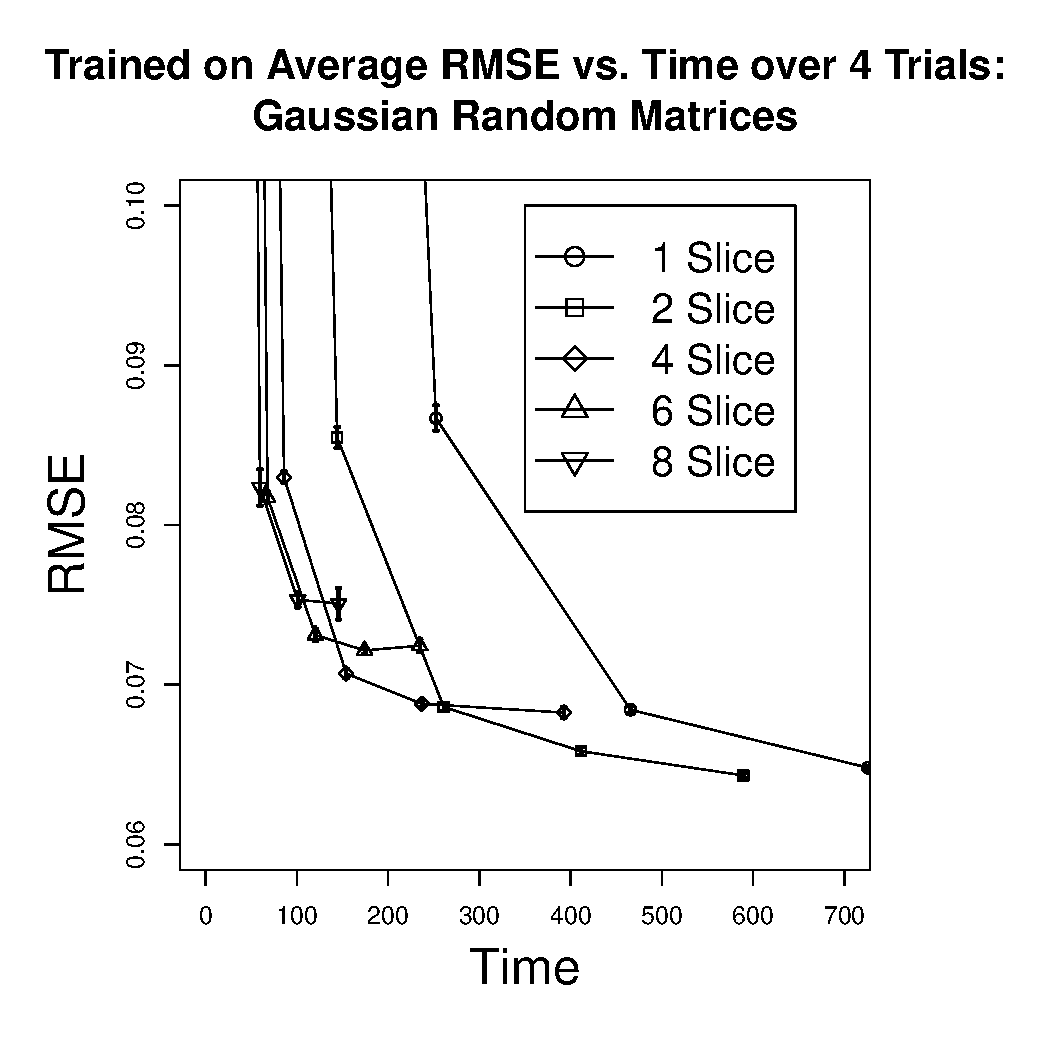
\includegraphics[width=\textwidth]{Graphs/4000_90_1_to_4_RvT_graph.pdf}}
		\caption{Training Data.}
\end{center}
	\end{subfigure}
\hspace{1cm}
	\begin{subfigure}[b]{.45\textwidth}
\begin{center}
		\fbox{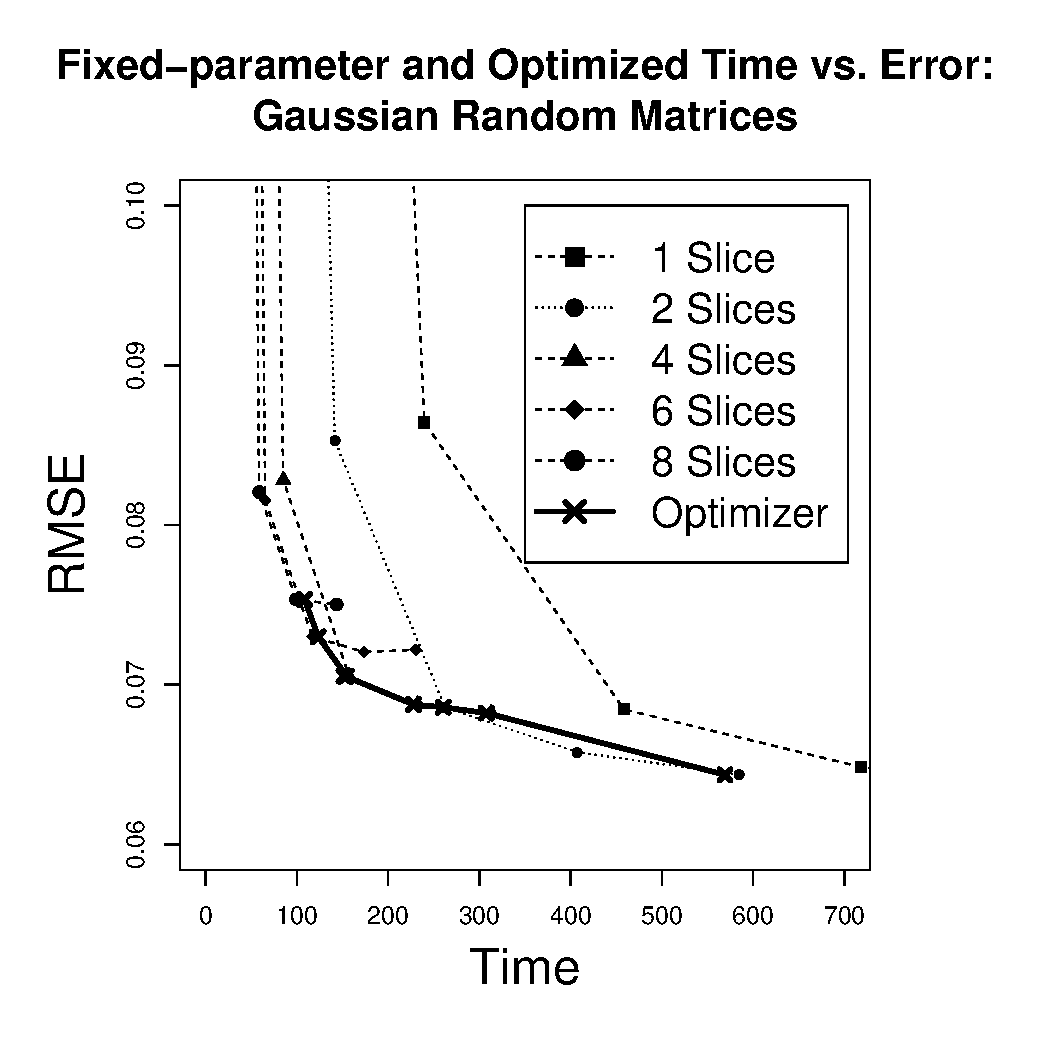
\includegraphics[width=\textwidth]{Graphs/Opt_Gaussian_4000.pdf}}
		\caption{Testing Data.}
\end{center}
	\end{subfigure}
\hfill
	\caption{Plots of vs. Time Error taken to factor a 4000 by 4000 
	low-rank matrix drawn from a Gaussian distribution. The choices of the 
	optimizer are indicated in the testing plot.}	

\end{figure*}

\subsection{Movielens Data}
The second dataset we used to test the optimizer was the Movielens10M 
dataset. The Movielens dataset is a set of entries 
$(\text{UserID},\text{MovieID},\text{rating})$, with the rating 
parameter being a half-integer between $1$ and $5$. One can think of 
these tuples as specifying the entries of a matrix with rows 
and columns indexed by users and movies. 

The reason we might want to find a low-rank completion of this matrix 
is the assumption that there are a small number of properties that 
influence the way people rate movies. Then the two factors tell you 
how a person values each property, and how each movie is correlated 
with these properties. This lets you make predictions even on the 
hidden entries of the matrix, i.e. the movies a user has yet to 
see or rate. 

There are some qualitative differences between this data and the 
synthetic data in the previous section. The entries come from 
the range $[1,5]$ rather than being concentrated around zero, 
and thus the RMSE's for this section are much larger. The 
Gaussian matrices also come from a well-understood distribution; this
means we can make theoretical guarantees about the behavior of  DFC 
on these instances, and also that it behaves pretty consistently across 
different random matrices. In the Movieens10M set we have no such 
guarantee, but under the assumption that the order of people is randomized,
we can hope that Movielens users behave similarly across partitions. 

The dataset was partitioned by the UserID into seven different 
pieces and the pieces were grouped to form the training/testing 
splits mentioned in the first section. Figure \ref{fig:movietraintest} 
displays the optimizer's performance on one of these splits. As before, 
each curve represents one of the choices of the division parameter in DFC. 
Once again we observe the intersection points where the division 
parameter should be changed for optimality to be satisfied. The bold 
line represents the optimized parameters for each budget. The graphs 
here are qualitatively the same as the graphs from the previous section. 
For every time budget, the optimizer picks the best division parameter. 

Table \ref{fig:MovieCrossTable} summarizes the results of each of the 
training/testing splits for the Movielens dataset. Averaged over 
all these splits, the optimized parameter choices perform within 
$2\%$ over the minimal error, and coming 
within $3\%$ over the budget.

\begin{table}
\label{fig:MovieCrossTable}
\begin{center}
    \begin{tabular}{| p{2.2cm} | p{2.2cm} | p{2.2cm} |}
    \hline
    Testing Set & \% Over Optimal Error & \% Over Time Budget \\ \hline
    1 & 2.0\% & -11.9\% \\ \hline
    2 & 0.1\% & -10.9\% \\ \hline
    3 & -1.8\% & -10.2\% \\ \hline
    4 & -1.0\% & -9.3\% \\ \hline
    5 & 1.1\% & -10.5\% \\ \hline
    6 & 0.9\% & -14.9\% \\ \hline
    7 & -2.9\% & 2.3\% \\ \hline
    \end{tabular}
\end{center}
\caption{Average regret and time for k-fold cross-validation of optimizer run on the seven Movielens matrices. Percentages are in relationship to best possible error and time budget respectively.}
\end{table}

\begin{figure*}
\label{fig:movietraintest}
	\begin{subfigure}[b]{.45\textwidth}
\begin{center}
		\fbox{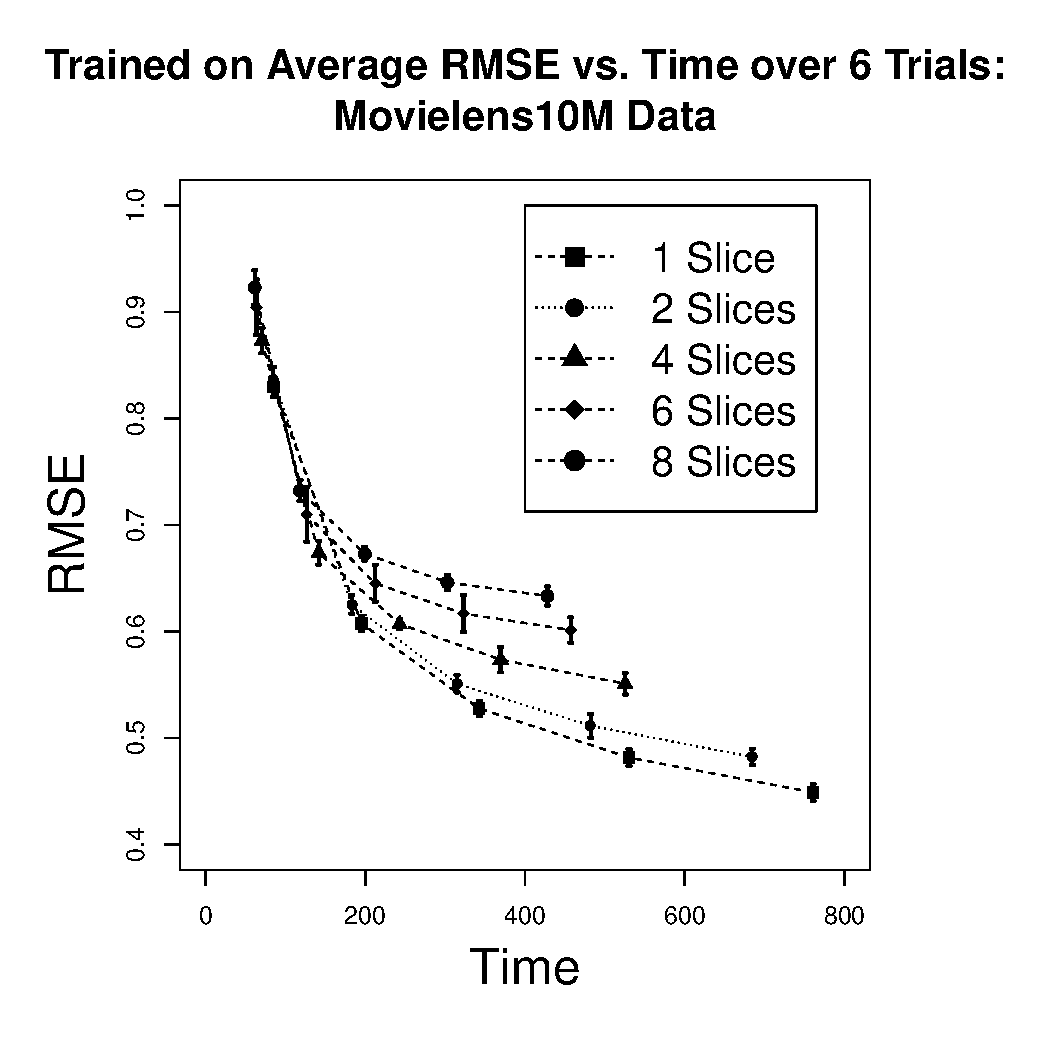
\includegraphics[width=\textwidth]{Graphs/movielens10M_1_to_4_RvT_graph.pdf}}
		\caption{Training Data.}
\end{center}
	\end{subfigure}
\hspace{1cm}
	\begin{subfigure}[b]{.45\textwidth}
\begin{center}
		\fbox{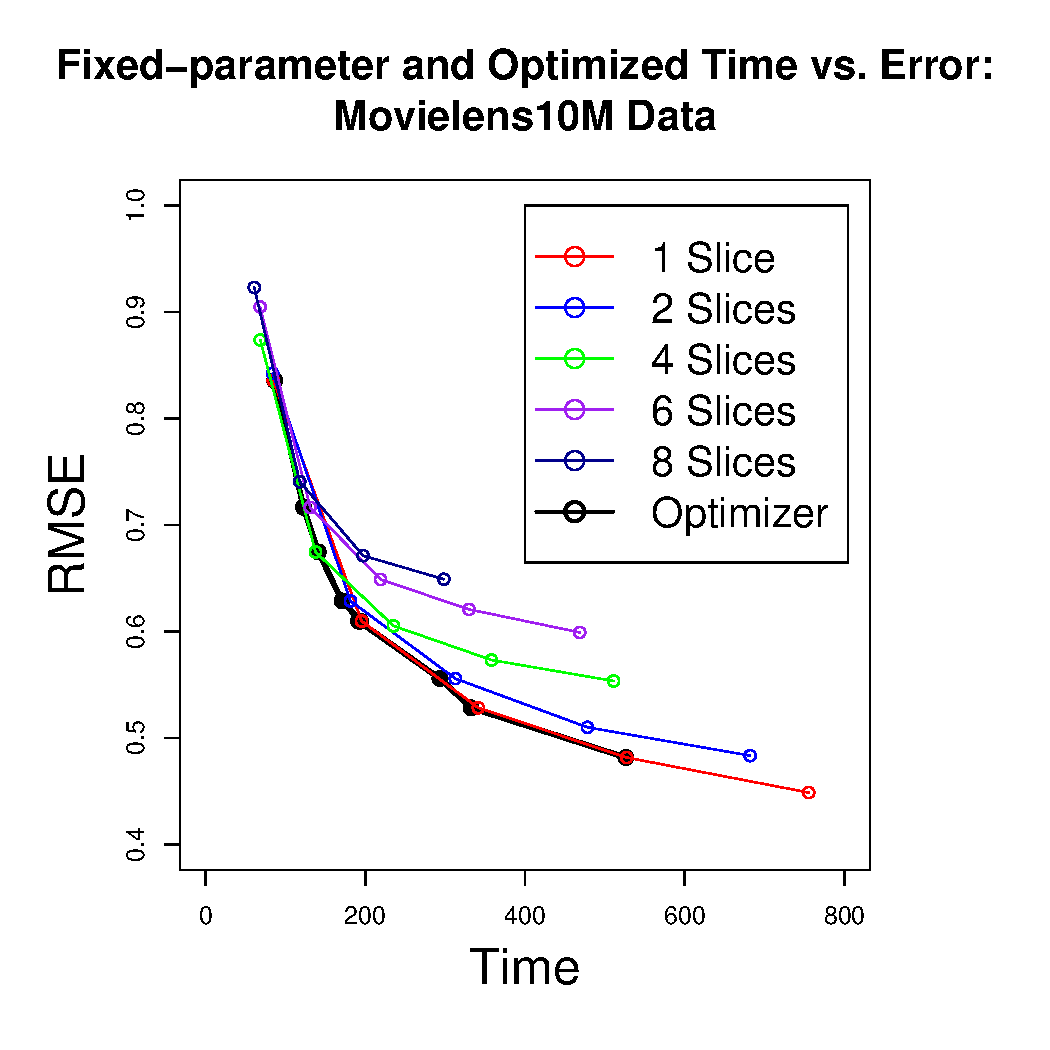
\includegraphics[width=\textwidth]{Graphs/Opt_movielens.pdf}}
		\caption{Testing Data. }
\end{center}
	\end{subfigure}
\hfill
	\caption{Plots of Time vs. Error taken to factor the Movielens10M 
	Dataset partitions. The optimizer's choices are shown on the testing
	plot.}	

\end{figure*}

\subsection{Training with Limited Data}
In an effort to discover how much training data we need for accurate 
optimizer predictions, we also ran some tests on training/testing 
splits with smaller training sets. Instead of training on six 
data partitions, we tried training the optimizer on only two partitions 
and testing it on the remaining five. The optimizer performs basically 
as well as if we had trained on almost all the partitions. 
Table \ref{fig:MovieTrain2Table} summarizes these results. We believe 
this is because the data is qualitatively the same across all the 
partitions, so the additional partitions do not add a lot of information 
to the optimizer. Distributions with higher variance in behavior 
may require significantly more learning, though we have not yet 
tested this. 

\begin{table}
\label{fig:MovieTrain2Table}
\begin{center}
    \begin{tabular}{| p{2.2cm} | p{2.2cm} | p{2.2cm} |}
    \hline
    Testing Set & \% Over Optimal Error & \% Over Time Budget \\ \hline
    1 & -1.8\% & -10.5\% \\ \hline
    2 & -1.1\% & -11.7\% \\ \hline
    3 & 1.1\% & -12.0\% \\ \hline
    4 & 0.02\% & -13.9\% \\ \hline
    5 & -2.9\% & 2.29\% \\ \hline
    \end{tabular}
\end{center}
\caption{Average pecent regret and time for k-fold cross-validation of optimizer run on the seven Movielens matrices. Percentages are in relationship to best possible error and time budget respectively.}
\end{table}

\subsection{Testing Explore and Estimation Modes}
\label{sec:estEval}
The previous sections show that our optimizer performs quite well 
when the training set accurately reflects the behavior of the algorithm 
on the parameter space of future jobs. However, sometimes an 
application can receive an instance that is unlike the previously 
seen jobs. For example, a matrix from the same distribution with more
revealed entries could take more time to process (this is a realistic
example for recommender systems, in which the users add more and more
ratings to the system). In this case, we want to estimate  the computational
costs in the unknown regions of the parameter space, and to use some 
randomness while picking our parameters so that we can adjust our estimates
about the parameter space to reflect reality. 
Ideally, the optimizer will complete the estimate and explore phase 
without sacrificing too much in the error or time of the computation, 
so we pick parameters proportionally to the error we expect to get 
with those settings. 

We tested this functionality in the setting where the size of the problem
instance changes. To do this, we gave the optimizer training data from 
$2000 \times 2000$ Gaussian random matrices, and applied our estimation 
mode to guess runtime profiles for $4000 \times 4000$ Gaussian 
random matrices. Then, we gave the optimizer a sequence of 
ten $4000 \times 4000$ Gaussian random matrices and asked the 
computation to finish within 200 seconds. While exploring, 
the optimizer was able to find a parameter setting with an error 
that was within $15\%$ of the best parameter choice that satisfies 
that budget that we could find in hindsight. It did not find better 
settings because we over-estimated the amount of time per iteration, 
and so the optimizer did not try running with more iterations because 
it thought that would violate the budget. This is a problem that could be
much improved with better models for time per iteration, as discussed
in the conclusion.

\begin{table*}
\label{fig:4kAdaptiveTable}
\begin{center}
    \begin{tabular}{| p{2.2cm} | p{2.2cm} | p{2.2cm} | p{2.2cm} | p{2.2cm} |}
    \hline
    Test Matrix & RMSE & Running Time (sec) & Slices & Iterations \\ \hline
    1 & 0.26 & 41.7 & 4 & 10 \\ \hline
    2 & 0.27 & 37.0 & 5 & 10 \\ \hline
    3 & 0.08 & 67.7 & 6 & 20 \\ \hline
    4 & 0.08 & 74.8 & 5 & 20 \\ \hline
    5 & 0.26 & 70.0 & 2 & 10 \\ \hline
    6 & 0.09 & 239 & 1 & 20 \\ \hline
    7 & 0.26 & 124 & 1 & 10 \\ \hline
    8 & 0.26 & 50.8 & 3 & 10 \\ \hline
    9 & 0.27 & 33.7 & 7 & 10 \\ \hline
    10 & 0.09 & 140 & 2 & 20 \\ \hline
    \end{tabular}
\end{center}
\caption{Parameter choices and results for running the optimizer in explore and estimation modes on ten Gaussian random 4000 by 4000 matrices, using
data from 2000 by 2000 Gaussian matrices.}
\end{table*}
